\index{OpenQuake-engine!risk}

The seismic risk results are being calculated using the OpenQuake risk library
(oq-risklib), an open-source suite of tools for seismic risk assessment and
loss estimation. This library is written in the Python programming language
and available in the form of a ``developers'' release, that can be executed
through a command line interface. The code of the library can be found on a
public repository at GitHub at the following address
\href{http://github.com/gem/oq-risklib}{http://github.com/gem/oq-risklib}.

The risk component of the OpenQuake-engine can compute both scenario-based and
probabilistic seismic damage and risk using various approaches. The following
types of analysis are currently supported:

\begin{itemize}

    \item \textit{Scenario Damage Assessment}, allowing the calculation of
	damage distribution statistics for a portfolio of buildings from a single
	earthquake rupture scenario taking into account aleatory and epistemic
	ground-motion variability.

	\item \textit{Scenario Risk Assessment}, for the calculation of individual 
	asset and portfolio loss statistics due to a single earthquake 
	rupture scenario taking into account aleatory and epistemic ground-motion 
	variability. Correlation in the vulnerability of different assets of the 
	same typology can also be taken into consideration.

	\item \textit{Classical Probabilistic Seismic Damage Analysis}, for 
	calculation of damage state probabilities over a specified time period,  
	and probabilistic collapse maps, starting from the hazard curves 
	computed following the classical integration procedure (\cite{cornell1968}, 
	\citet{mcguire1976}) as formulated by \cite{field2003}.

    \item \textit{Classical Probabilistic Seismic Risk Analysis}, allowing
	calculation of loss curves and loss maps, starting from the hazard curves 
	computed following the classical integration procedure (\cite{cornell1968}, 
	\citet{mcguire1976}) as formulated by \cite{field2003}.

	\item \textit{Event-Based Probabilistic Seismic Risk Analysis}, 
	allowing calculation of event-loss tables starting from stochastic event sets.
	Other results such as loss-exceedance curves, probabilistic loss maps, 
	average annual losses, and insured loss statistics can be obtained by post-
	processing the event-loss tables.

	\item \textit{Retrofit Benefit-Cost Ratio Analysis}, which is useful in 
	estimating the net-present value of the potential benefits of performing  
	retrofitting for a portfolio of assets (in terms of decreased losses in 
	seismic events), measured relative to the upfront cost of retrofitting.

\end{itemize}

Each calculation workflow has a modular structure, so that intermediate
results can be exported and analyzed. Moreover, each calculator can be
extended independently of the others so that additional calculation options
and methodologies can be easily introduced, without affecting the overall
calculation workflow.

The following sections describe the basic inputs required for a risk
calculation, including exposure models, fragility models, consequence models,
and vulnerability models. The final section of this chapter describes each of
the above workflows in detail.

For further information regarding the theoretical background of the
methodologies used for each calculator, users are referred to the OpenQuake-
engine Book (Risk).


\section{Exposure models}
\label{sec:exposure}
All risk calculators in the OpenQuake-engine require an \gls{exposure model} that needs to be stored in NRML. There are a number of parameters that compose the metadata, and provides general information regarding the \glspl{asset} within the \gls{exposure model}, as described below:

\begin{itemize}
\item  \Verb+id+: a unique key used to identify the \gls{exposure model};
\item  \Verb+category+: a string used to define the type of \glspl{asset} being stored (e.g: buildings, population, contents);
\item  \Verb+taxonomySource+: attribute used to define the \gls{taxonomy} being used to classify the  \glspl{asset};
\item  \Verb+description+: brief string with further information about the \gls{exposure model};
\end{itemize}

This information is common to all the assets and needs to be incorporated at the beginning of the exposure model file according to the following example:

\begin{Verbatim}[frame=single, commandchars=\\\{\}, samepage=false]
<?xml version="1.0" encoding="UTF-8"?>
<nrml xmlns="http://openquake.org/xmlns/nrml/0.4">
<\textcolor{red}{exposureModel} id="exposure_model"
      category="buildings"
      taxonomySource="GEM taxonomy">
    <\textcolor{green}{description}>Buildings in Pavia</\textcolor{green}{description}>
...
\end{Verbatim}

The NRML schema for the exposure model allows the definition of various types of costs (structural cost, nonstructural cost, contents cost, business interruption cost). Further explanations regarding the quantities that are currently being used to define the exposure elements can be found in the OpenQuake-engine Book (Risk).

The way the information about the characteristics of the \glspl{asset} in an \gls{exposure model} are stored can vary strongly depending on how and why the data was compiled. As an example, if national census information is used to estimated the distribution of assets in a given region, it is likely that the number of buildings within a given geographical area will be used to define the dataset, and will be used for estimating the number of collapsed buildings for a scenario earthquake. On the other hand, if simplified methodologies based on proxy data such as population distribution are used to develop the exposure model, then it is likely that the built up area or economic cost of each building typology will be directly derived, and will be used for the estimation of economic losses. Thus, the following set of attributes exist within the schema for the exposure model:

\begin{itemize}
\item  \Verb+number+: number of units of a given \gls{asset} at a given location;
\item  \Verb+area+: area of the \gls{asset}, at a given location;
\item  \Verb+cost+: structural replacement cost of the \gls{asset} at a given location;
\end{itemize}

The set of required attributes depends on what and how a user wants to store the information about the assets in the exposure model. While the attribute \Verb+number+ might be a rather simple parameter, the other two (area and cost) can be ambiguous, as different ways to define them might be used. With regards to the attribute \Verb+area+, one can either choose to provide the aggregated built up area of the \glspl{asset} per location or the average built up area for a single building unit (noting that an \gls{asset} might be made up of a number of individual buildings). Similarly, the \Verb+cost+ can also be defined as the aggregated structural replacement cost, the cost of replacing a single unit or even the structural replacement cost per unit of area. For the purposes of performing a retrofitting benefit/cost analysis, it is also necessary to define the retrofitting cost (\Verb+reco+). The combination between the possible options in which these three attributes can be defined leads to four ways of storing the information about the assets. For each of these cases a brief explanation and example is provided in this section.

\paragraph{Example 1}
This example is comprised of an \gls{exposure model} in which the aggregated cost (structural, nonstructural, contents and business interruption) of the buildings of each taxonomy for a set of locations is directly provided. Thus, in order to indicate how the various costs will be defined, the following information needs to be stored in the exposure model file:

\begin{Verbatim}[frame=single, commandchars=\\\{\}, samepage=false]
...
 <\textcolor{green}{conversions}>
  <\textcolor{blue}{costTypes}>
   <\textcolor{magenta}{costType} name="structural" type="aggregated" unit="EUR">
   <\textcolor{magenta}{costType} name="non_structural" type="aggregated" unit="EUR" />
   <\textcolor{magenta}{costType} name="business_interruption" type="aggregated" 
                                                      unit="EUR"/>
   <\textcolor{magenta}{costType} name="contents" type="aggregated" unit="EUR"/>
  </\textcolor{blue}{costTypes}>
 </\textcolor{green}{conversions}>
...
\end{Verbatim}

In this case, the cost \Verb+type+ of each component as been defined as \Verb+aggregated+. Once the way in which each cost is going to be defined has been established, the values for each asset can be stored according to the following format:

\begin{Verbatim}[frame=single, commandchars=\\\{\}, samepage=false]
...
 <\textcolor{green}{assets}>
  <\textcolor{blue}{asset} id="asset_01" taxonomy="RC/DMRF-D/LR">
   <\textcolor{magenta}{location} lon="9.15" lat="45.17" />
   <\textcolor{magenta}{costs}>
    <cost type="structural" value="1500"/>
    <cost type="non_structural" value="2500"/>
    <cost type="contents" value="1200"/>
    <cost type="business_interruption" value="400"/>
   </\textcolor{magenta}{costs}>
  </\textcolor{blue}{asset}>
...
  <\textcolor{blue}{asset} id="asset_99"  taxonomy="RC/DMRF-D/HR">
   <\textcolor{magenta}{location} lon="9.15" lat="45.12" />
   <\textcolor{magenta}{costs}>
    <cost type="structural" value="2500"/>
    <cost type="non_structural" value="2100"/>
    <cost type="contents" value="1900"/>
    <cost type="business_interruption" value="40"/>
   </\textcolor{magenta}{costs}>
  </\textcolor{blue}{asset}>
 </\textcolor{green}{assets}>
</\textcolor{red}{exposureModel}>
</nrml>
\end{Verbatim}

Each \gls{asset} is uniquely identified by its \Verb+id+, which is used by the OpenQuake-engine to relate each asset with the associated results (e.g. loss exceedance curves). Then, a pair of coordinates (latitude and longitude) for a \Verb+location+ where the asset is assumed to exist is defined. \footnote{Within the OpenQuake-engine, longitude and latitude coordinates are internally rounded to a precision of 5 digits after the decimal point.} Each asset must be classified according to a \Verb+taxonomy+, so that the OpenQuake-engine is capable of employing the appropriate \gls{vulnerability function} or \gls{fragility function} in the risk calculations. Finally, the cost values of each \Verb+type+ are stored within the \Verb+costs+ attribute. In this example, the aggregated value for all units (within a given asset) at each location is provided directly, so there is no need to define other attributes such as \Verb+number+ or \Verb+area+. This mode of representing an exposure model is probably the simplest one.

\paragraph{Example 2}
In this example an \gls{exposure model} containing the number of units (buildings) and the associated costs per unit of each building typology is presented.

\begin{Verbatim}[frame=single, commandchars=\\\{\}, samepage=false]
...
 <\textcolor{green}{conversions}>
  <\textcolor{blue}{costTypes}>
   <\textcolor{magenta}{costType} name="structural" type="per_unit" unit="EUR">
   <\textcolor{magenta}{costType} name="non_structural" type="per_unit" unit="EUR" />
   <\textcolor{magenta}{costType} name="business_interruption" type="per_unit" 
                                                      unit="EUR"/>
   <\textcolor{magenta}{costType} name="contents" type="per_unit" unit="EUR"/>
  </\textcolor{blue}{costTypes}>
 </\textcolor{green}{conversions}>
...
\end{Verbatim}

For this case, the cost \Verb+type+ has been set to \Verb+per_unit+. Then, the information from each asset can be stored following the format below:

\begin{Verbatim}[frame=single, commandchars=\\\{\}, samepage=false]
...
 <\textcolor{green}{assets}>
  <\textcolor{blue}{asset} id="asset_01" number="10" taxonomy="RC/DMRF-D/LR">
   <\textcolor{magenta}{location} lon="9.15" lat="45.17" />
   <\textcolor{magenta}{costs}>
    <cost type="structural" value="150"/>
    <cost type="non_structural" value="250"/>
    <cost type="contents" value="120"/>
    <cost type="business_interruption" value="40"/>
   </\textcolor{magenta}{costs}>
  </\textcolor{blue}{asset}>
...
  <\textcolor{blue}{asset} id="asset_99" number="20" taxonomy="RC/DMRF-D/HR">
   <\textcolor{magenta}{location} lon="9.15" lat="45.12" />
   <\textcolor{magenta}{costs}>
    <cost type="structural" value="125"/>
    <cost type="non_structural" value="105"/>
    <cost type="contents" value="95"/>
    <cost type="business_interruption" value="20"/>
   </\textcolor{magenta}{costs}>
  </\textcolor{blue}{asset}>
 </\textcolor{green}{assets}>
</\textcolor{red}{exposureModel}>
</nrml>
\end{Verbatim}

In this example, the various costs for each asset is not provided directly, as happened in the previous example. In order to carry out the risk calculations in which the economic cost of each asset is required, the OpenQuake-engine multiplies, for each asset, the number of units (buildings) by the ``per unit'' replacement cost. Note that in this case, there is no need to specify the attribute \Verb+area+.

\paragraph{Example 3}
This example is comprised of an \gls{exposure model} containing the built up area of each building typology for a set of locations, and the associated costs per area.

\begin{Verbatim}[frame=single, commandchars=\\\{\}, samepage=false]
...
 <\textcolor{green}{conversions}>
  <\textcolor{blue}{area} type="aggregated" unit="square meters"/>
  <\textcolor{blue}{costTypes}>
   <\textcolor{magenta}{costType} name="structural" type="per_area" unit="EUR">
   <\textcolor{magenta}{costType} name="non_structural" type="per_area" unit="EUR" />
   <\textcolor{magenta}{costType} name="business_interruption" type="per_area" 
                                                      unit="EUR"/>
   <\textcolor{magenta}{costType} name="contents" type="per_area" unit="EUR"/>
  </\textcolor{blue}{costTypes}>
 </\textcolor{green}{conversions}>
...
\end{Verbatim}

In order to compile an \gls{exposure model} with this structure, it is required to set the cost \Verb+type+ to \Verb+per_area+. In addition, it is also necessary to specify if the \Verb+area+ that is being store represents the aggregated area of number of units within an asset, or the average area of a single unit. In this particular case, the \Verb+area+ that is being stored is the aggregated built up area per asset, and thus this attribute was set to \Verb+aggregated+.

\begin{Verbatim}[frame=single, commandchars=\\\{\}, samepage=false]
...
 <\textcolor{green}{assets}>
  <\textcolor{blue}{asset} id="asset_01" area="50" taxonomy="RC/DMRF-D/LR">
   <\textcolor{magenta}{location} lon="9.15" lat="45.17" />
   <\textcolor{magenta}{costs}>
    <cost type="structural" value="100"/>
    <cost type="non_structural" value="200"/>
    <cost type="contents" value="90"/>
    <cost type="business_interruption" value="10"/>
   </\textcolor{magenta}{costs}>
  </\textcolor{blue}{asset}>
...
  <\textcolor{blue}{asset} id="asset_99" area ="60" taxonomy="RC/DMRF-D/HR">
   <\textcolor{magenta}{location} lon="9.15" lat="45.12" />
   <\textcolor{magenta}{costs}>
    <cost type="structural" value="150"/>
    <cost type="non_structural" value="250"/>
    <cost type="contents" value="50"/>
    <cost type="business_interruption" value="30"/>
   </\textcolor{magenta}{costs}>
  </\textcolor{blue}{asset}>
 </\textcolor{green}{assets}>
</\textcolor{red}{exposureModel}>
</nrml>
\end{Verbatim}

Once again, the OpenQuake-engine needs to carry out some calculations in order to compute the different costs per asset. In this case, this value is computed by multiplying the aggregated built up \Verb+area+ of each building typology by the associated cost per unit of area. Notice that in this case, there is no need to specify the attribute \Verb+number+.

\paragraph{Example 4}
This example is comprised of an \gls{exposure model} containing the number of buildings for each location, the average built up area per building unit and the associated costs per area.

\begin{Verbatim}[frame=single, commandchars=\\\{\}, samepage=false]
...
 <\textcolor{green}{conversions}>
  <\textcolor{blue}{area} type="per_asset" unit="square meters"/>
  <\textcolor{blue}{costTypes}>
   <\textcolor{magenta}{costType} name="structural" type="per_area" unit="EUR">
   <\textcolor{magenta}{costType} name="non_structural" type="per_area" unit="EUR" />
   <\textcolor{magenta}{costType} name="business_interruption" type="per_area" 
                                                      unit="EUR"/>
   <\textcolor{magenta}{costType} name="contents" type="per_area" unit="EUR"/>
  </\textcolor{blue}{costTypes}>
 </\textcolor{green}{conversions}>
...
\end{Verbatim}

Similarly to what was described in the previous example, the various costs \Verb+type+ also need to be establish as \Verb+per_area+, but the \Verb+type+ of area is now defined as \Verb+per_unit+.

\begin{Verbatim}[frame=single, commandchars=\\\{\}, samepage=false]
...
 <\textcolor{green}{assets}>
  <\textcolor{blue}{asset} id="asset_01" number="5" area="50" taxonomy="RC/DMRF-D/LR">
   <\textcolor{magenta}{location} lon="9.15" lat="45.17" />
   <\textcolor{magenta}{costs}>
    <cost type="structural" value="100"/>
    <cost type="non_structural" value="200"/>
    <cost type="contents" value="90"/>
    <cost type="business_interruption" value="10"/>
   </\textcolor{magenta}{costs}>
  </\textcolor{blue}{asset}>
...
  <\textcolor{blue}{asset} id="asset_99" number="8" area ="60" taxonomy="RC/DMRF-D/HR">
   <\textcolor{magenta}{location} lon="9.15" lat="45.12" />
   <\textcolor{magenta}{costs}>
    <cost type="structural" value="150"/>
    <cost type="non_structural" value="250"/>
    <cost type="contents" value="50"/>
    <cost type="business_interruption" value="30"/>
   </\textcolor{magenta}{costs}>
  </\textcolor{blue}{asset}>
 </\textcolor{green}{assets}>
</\textcolor{red}{exposureModel}>
</nrml>
\end{Verbatim}

In this example, the OpenQuake-engine will make use of all the parameters to estimate the various costs of each asset, by multiplying the number of buildings by its average built up area, and then by the respective cost per unit of area.

\paragraph{Example 5}
In this example, additional information will be included, which is required for other risk analysis besides loss estimation, such as the calculation of insured losses or benefit/cost analysis. For the former assessment, it is necessary to establish how the insured limit and deductible is going to be define, according to the format below. 
\begin{Verbatim}[frame=single, commandchars=\\\{\}, samepage=false]
...
 <\textcolor{green}{conversions}>
  <\textcolor{blue}{costTypes}>
   <\textcolor{magenta}{costType} name="structural" type="aggregated" unit="EUR">
   <\textcolor{magenta}{costType} name="non_structural" type="aggregated" unit="EUR" />
   <\textcolor{magenta}{costType} name="business_interruption" type="aggregated" 
                                                      unit="EUR"/>
   <\textcolor{magenta}{costType} name="contents" type="aggregated" unit="EUR"/>
  </\textcolor{blue}{costTypes}>
  <\textcolor{blue}{deductible} isAbsolute="false"/>
  <\textcolor{blue}{insuranceLimit} isAbsolute="false"/>
 </\textcolor{green}{conversions}>
...
\end{Verbatim}

In this example, both the insurance limit and the deductible were defined as a fraction of the costs, by setting the attribute \Verb+isAbsolute+ to \Verb+false+. On the other hand, a user could define one or both of these parameters as the absolute threshold, by setting the aforementioned attribute to \Verb+true+. Then, for each type of cost, the limit and deductible value can be stored for each asset.
Moreover, in order to perform a benefit/cost assessment, it is also fundamental to indicate the retrofitting cost. This parameter is handled in the same manner as the structural cost, and it should be stored according to the following structure.

\begin{Verbatim}[frame=single, commandchars=\\\{\}, samepage=false]
...
 <\textcolor{green}{assets}>
  <\textcolor{blue}{asset} id="asset_01" taxonomy="RC/DMRF-D/LR">
   <\textcolor{magenta}{location} lon="9.15" lat="45.17" />
   <\textcolor{magenta}{costs}>
    <cost type="structural" value="1500" deductible=".05" 
                insuranceLimit="0.9" retrofitted="200"/>
    <cost type="non_structural" value="2500" deductible=".1" 
                insuranceLimit="0.8"/>
    <cost type="contents" value="1200" deductible=".2" 
                insuranceLimit="0.6"/>
    <cost type="business_interruption" value="400" deductible=".1" 
                insuranceLimit="0.5"/>
   </\textcolor{magenta}{costs}>
  </\textcolor{blue}{asset}>
...
  <\textcolor{blue}{asset} id="asset_99"  taxonomy="RC/DMRF-D/HR">
   <\textcolor{magenta}{location} lon="9.15" lat="45.12" />
   <\textcolor{magenta}{costs}>
    <cost type="structural" value="2500" deductible=".1" 
                insuranceLimit="0.9"/ retrofitted="300"/>
    <cost type="non_structural" value="2100" deductible=".05" 
                insuranceLimit="0.7"/>
    <cost type="contents" value="1900" deductible=".2" 
                insuranceLimit="0.7"/>
    <cost type="business_interruption" value="40"/ deductible=".05" 
                insuranceLimit="0.9">
   </\textcolor{magenta}{costs}>
  </\textcolor{blue}{asset}>
 </\textcolor{green}{assets}>
</\textcolor{red}{exposureModel}>
</nrml>
\end{Verbatim}

Despite the fact that for the demonstration of how the insurance parameters and retrofitting cost can be stored it was used the aggregated type of cost (structure described in example 1), it is important to mention that any of the other storing approaches can also be employed (example 2 -4).

\paragraph{Example 6}
The OpenQuake-engine is also capable of estimating human losses, based on a number of occupants within an asset, at a certain time of the day. In this example, it is demonstrated how this parameter is defined for each asset. In addition, this example also serves the purpose of presenting an \gls{exposure model} in which three cost types have been defined following different structures.

\begin{Verbatim}[frame=single, commandchars=\\\{\}, samepage=false]
...
 <\textcolor{green}{conversions}>
  <\textcolor{blue}{area} type="aggregated" unit="square meters"/>
  <\textcolor{blue}{costTypes}>
   <\textcolor{magenta}{costType} name="structural" type="per_unit" unit="EUR">
   <\textcolor{magenta}{costType} name="non_structural" type="per_area" unit="EUR" />
   <\textcolor{magenta}{costType} name="contents" type="aggregated" unit="EUR"/>
  </\textcolor{blue}{costTypes}>
 </\textcolor{green}{conversions}>
...
\end{Verbatim}

As previously mentioned, in this example only three costs are being stored, and each one follows a different approach. The \Verb+structural+ cost is being defined as the replacement cost per unit (example 2), the \Verb+non_structural+ cost is established as the cost per area (example 3), and the \Verb+contents+ cost is provided directly as the aggregated value per asset (example 1). The information about each asset is presented bellow, along with the number of occupants at different times of the day.

\begin{Verbatim}[frame=single, commandchars=\\\{\}, samepage=false]
...
 <\textcolor{green}{assets}>
  <\textcolor{blue}{asset} id="asset_01" number="5" area ="500" taxonomy="RC/DMRF-D/LR">
   <\textcolor{magenta}{location} lon="9.15" lat="45.17" />
   <\textcolor{magenta}{costs}>
    <cost type="structural" value="1000"/>
    <cost type="non_structural" value="250"/>
    <cost type="contents" value="5000"/>
   </\textcolor{magenta}{costs}>
   <\textcolor{magenta}{occupancies}>
    <occupancy occupants="10" period="day"/>
    <occupancy occupants="50" period="night"/>
   </\textcolor{magenta}{occupancies}>
  </\textcolor{blue}{asset}>
...
  <\textcolor{blue}{asset} id="asset_99" number="8" area ="800" taxonomy="RC/DMRF-D/HR">
   <\textcolor{magenta}{location} lon="9.15" lat="45.12" />
   <\textcolor{magenta}{costs}>
    <cost type="structural" value="2000"/>
    <cost type="non_structural" value="400"/>
    <cost type="contents" value="4000"/>
   </\textcolor{magenta}{costs}>
   <\textcolor{magenta}{occupancies}>
    <occupancy occupants="20" period="day"/>
    <occupancy occupants="30" period="night"/>
   </\textcolor{magenta}{occupancies}>
  </\textcolor{blue}{asset}>
 </\textcolor{green}{assets}>
</\textcolor{red}{exposureModel}>
</nrml>
\end{Verbatim}

The number of occupants for each asset is stored under the \Verb+occupancies+ field, as part of the \Verb+occupancy+ instance. The number and type of periods of the day is not a fixed variable, and a user can provide as many as needed (e.g. morning, afternoon, night, transit, 9am-17pm). The descriptions used to define each \Verb+period+ are used to specify the time of the day for which the human losses should be estimated in the Scenario Risk calculator.

The way this information is being stored is constantly being modified, as further feedback from users and experts is received. Hence, it is important to understand which version of NRML the engine is using, in order to avoid incompatibility issues. NRML is currenly v0.4 and documentation about each release can be found on GitHub (see \href{http://gitub.com/gem/oq-nrmllib}{oq-nrmllib}). Several examples of \glspl{exposure model} containing different types of information are presented below.

\section{Fragility models}
\label{sec:fragility}
This section describes the schema currently used to store \glspl{fragility
model}, which are required for the Scenario Damage Calculator and the
Classical Probabilistic Seismic Damage Calculator. A \gls{fragility model}
defines a set of \glspl{fragility function}, describing the probability of
exceeding a set of limit, or damage, states. These \gls{fragility function}
can be defined in two ways: discrete or continuous.

For discrete fragility functions, sets of probabilities of exceedance (one set
per limit state) are defined for a list of intensity measure levels, as
illustrated in Figure~\ref{fig:fragility-discrete}.

\begin{figure}[ht]
\centering
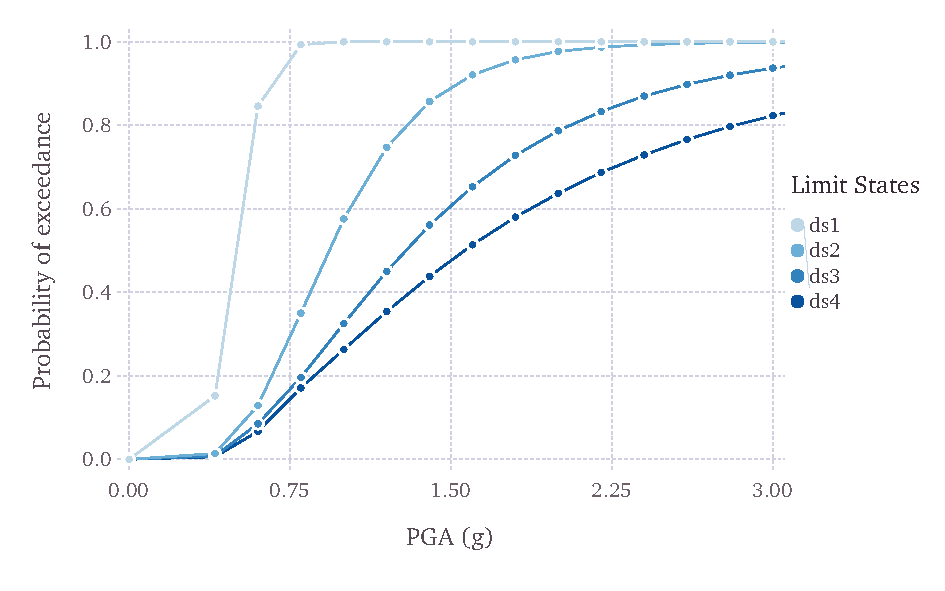
\includegraphics[width=12cm]{figures/risk/fragility-discrete.pdf}
\caption{Graphical representation of a discrete fragility model}
\label{fig:fragility-discrete}
\end{figure}

The \glspl{fragility function} can also be defined as continuous functions,
through the use of cumulative lognormal distribution functions. In
Figure~\ref{fig:fragility-continuous}, a continuous \gls{fragility model} is
presented.

\begin{figure}[ht]
\centering
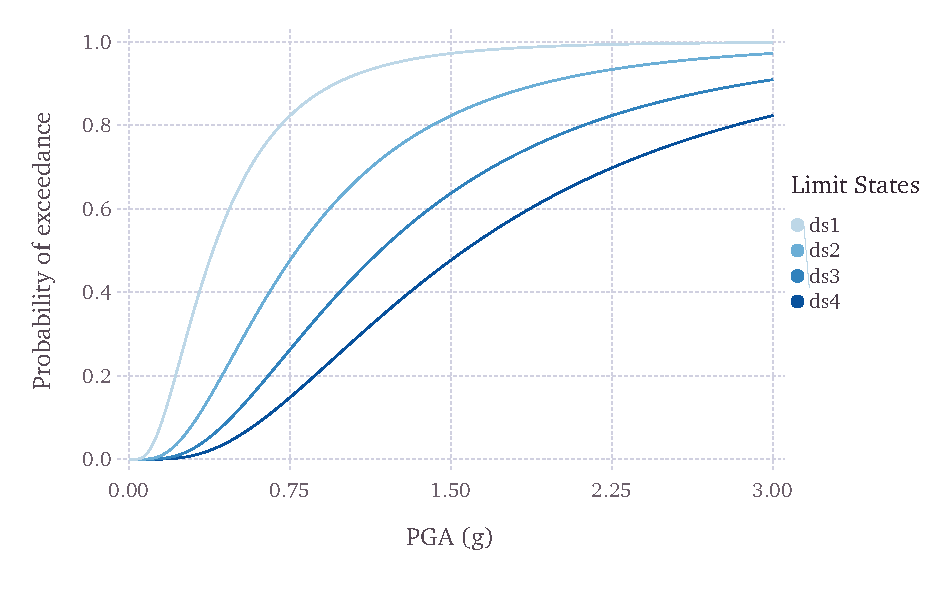
\includegraphics[width=12cm]{figures/risk/fragility-continuous.pdf}
\caption{Graphical representation of a continuous fragility model}
\label{fig:fragility-continuous}
\end{figure}

An example \gls{fragility model} comprising one discrete \gls{fragility
function} and one continuous \gls{fragility function} is shown below:

\inputminted[firstline=1,firstnumber=1,fontsize=\footnotesize,frame=single,linenos,bgcolor=lightgray]{xml}{oqum/risk/Verbatim/input_fragility.xml}\\


The initial portion of the schema contains general information that describes 
some general aspects of the \gls{fragility model}.

\begin{itemize}

    \item \Verb+id+: a unique key used to identify the \gls{fragility model}

    \item \Verb+assetCategory+: an optional string used to specify the type of
    \glspl{asset} for which \glspl{fragility function} will be defined in this
    file (e.g: buildings, lifelines)

    \item \Verb+lossCategory+: valid strings for this attribute are 
    ``structural'', ``nonstructural'', ``contents'', and 
    ``business\_interruption''

    \item \Verb+description+: a brief string with further information about the
    \gls{exposure model}

\end{itemize}

\inputminted[firstline=4,firstnumber=4,lastline=9,fontsize=\footnotesize,frame=single,linenos,bgcolor=lightgray]{xml}{oqum/risk/Verbatim/input_fragility.xml}\\

The information in the metadata section is common to all of the functions in
the \gls{fragility model} and needs to be included at the beginning of every
\gls{fragility model} file. The parameters are described below:

\begin{itemize}

    \item \Verb+description+: a brief string with further information about the
    \gls{fragility model}, for example, which building typologies are covered or 
    the source of the functions in the \gls{fragility model}

    \item \Verb+limitStates+: this field is used to define the number and 
    nomenclature of each limit state. Four limit states are employed in the 
    example above, but it is possible to use any number of discrete states,
    as long as a fragility curve is always defined for each limit state. The 
    limit states must be provided as a set of strings separated by whitespaces 
    between each limit state. Please ensure that there is no whitespace within 
    the name of any individual limit state.

\end{itemize}

In order to perform probabilistic or scenario damage calculations, it is
necessary to define a \gls{fragility function} for each building typology present in
the exposure model. The \glspl{fragility function} can be defined using either a
discrete or a continuous format, and the \gls{fragility model} file can include a
mix of both types of \glspl{fragility function}.

The following snippet from the above fragility model example file defines a
discrete fragility function:

\inputminted[firstline=11,firstnumber=11,lastline=17,fontsize=\footnotesize,frame=single,linenos,bgcolor=lightgray]{xml}{oqum/risk/Verbatim/input_fragility.xml}\\

The following attributes are needed to define a discrete \gls{fragility function}:

\begin{itemize}

    \item \Verb+id+: a unique key used to identify the \gls{taxonomy} for 
    which the function is being defined. This key is used to relate the 
    \gls{fragility function} with the relevant \gls{asset} in the 
    \gls{exposure model}.

    \item \Verb+format+: for discrete fragility functions, this attribute 
    should be set to ``\Verb+discrete+''

    \item \Verb+imls+: this attribute specifies the list of intensity levels
    for which the limit state probabilities of exceedance will be defined. 
    In addition, it is also necessary to define the intensity measure type 
    (\Verb+imt+). Optionally, a \Verb+noDamageLimit+ can be specified, which 
    defines the intensity level below which the probability of exceedance 
    for all limit states is taken to be zero.

    \item \Verb+poes+: this field is used to define the probabilities of 
    exceedance (\Verb+poes+) for each limit state for this 
    \gls{fragility function}. It is also necessary to specify which limit 
    state the exceedance probabilities are being defined for using the 
    attribute \Verb+ls+. The probabilities of exceedance for each limit state
    must be provided on a separate line; and the number of exceedance 
    probabilities for each limit state defined by the \Verb+poes+ attribute 
    must be equal to the number of intensity levels defined by the attribute 
    \Verb+imls+. Finally, the number and names of the limit states in each 
    fragility function must be equal to the number of limit states defined 
    earlier in the metadata section of the \gls{fragility model} using the 
    attribute \Verb+limitStates+.

\end{itemize}



The following snippet from the above \gls{fragility model} example file
defines a continuous \gls{fragility function}:

\inputminted[firstline=19,firstnumber=19,lastline=25,fontsize=\footnotesize,frame=single,linenos,bgcolor=lightgray]{xml}{oqum/risk/Verbatim/input_fragility.xml}\\

The following attributes are needed to define a continuous \gls{fragility function}:

\begin{itemize}

    \item \Verb+id+: a unique key used to identify the \gls{taxonomy} for 
    which the function is being defined. This key is used to relate the 
    \gls{fragility function} with the relevant \gls{asset} in the 
    \gls{exposure model}.

    \item \Verb+format+: for continuous fragility functions, this attribute 
    should be set to ``\Verb+continuous+''

    \item \Verb+shape+: for continuous fragility functions using the lognormal
    cumulative distrution, this attribute should be set to ``\Verb+logncdf+''.
    At present, only the lognormal cumulative distribution function can be 
    used for representing continuous fragility functions.

    \item \Verb+imls+: this element specifies various aspects related to the 
    intensity measure used by the the \gls{fragility function}. The range of 
    intensity levels for which the continuous fragility functions are valid 
    are specified using the attributes \Verb+minIML+ and \Verb+maxIML+. 
    In addition, it is also necessary to define the intensity measure type 
    \Verb+imt+. Optionally, a \Verb+noDamageLimit+ can be specified, which 
    defines the intensity level below which the probability of exceedance 
    for all limit states is taken to be zero.

    \item \Verb+params+: this field is used to define the parameters of 
    the (\Verb+params+) for each limit state for this 
    \gls{fragility function}. For a lognormal cumulative distrbution function, 
    the two parameters required to specify the function are the mean and 
    standard deviation of the intensity level. These parameters are defined for 
    each limit state using the attributes \Verb+mean+ and \Verb+stddev+ 
    respectively. The attribute \Verb+ls+ specifies the limit state for which 
    the parameters are being defined. The parameters for each limit state
    must be provided on a separate line. The number and names of the limit 
    states in each fragility function must be equal to the number of limit 
    states defined earlier in the metadata section of the \gls{fragility model}
    using the attribute \Verb+limitStates+.

\end{itemize}


Several methodologies to derive fragility functions are currently being
evaluated by \gls{acr:gem} and have been included as part of the Risk
Modeller's Toolkit, the code for which can be found on a public repository at
GitHub at the following address: 
\href{http://github.com/gemsciencetools/rmtk}{http://github.com/gemsciencetools/rmtk}.

Scripts to convert \glspl{fragility function} in CSV format or as Excel or
ASCII files into NRML are also under development, and can be found at the
OpenQuake platform at the following address:
\href{https://platform.openquake.org/risk_input_preparation_toolkit/}{https://platform.openquake.org/risk\_input\_preparation\_toolkit/}.


\section{Consequence models}
\label{sec:consequence}
Starting from OpenQuake-engine v1.6, the Scenario Damage calculator also
accepts consequence models in addition to fragility models, in order to
estimate consequences based on the calculated damage distribution. The user
may provide one consequence model file corresponding to each loss type
(amongst structural, nonstructural, contents, and business interruption) for
which a fragility model file is provided. Whereas providing a fragility model
file for at least one loss type is mandatory for running a Scenario Damage
calculation, providing corresponding consequence model files is optional.

This section describes the schema currently used to store \glspl{consequence
model}, which are optional inputs for the Scenario Damage Calculator. A
\gls{consequence model} defines a set of \glspl{consequence function},
describing the distribution of the loss (or consequence) ratio conditional on
a set of discrete limit (or damage) states. These \gls{consequence function}
can be currently defined in OpenQuake-engine by specifying the parameters of
the continuous distribution of the loss ratio for each limit state specified
in the fragility model for the corresponding loss type, for each taxonomy
defined in the exposure model.

An example consequence model is shown below:

\inputminted[firstline=1,firstnumber=1,fontsize=\footnotesize,frame=single,linenos,bgcolor=lightgray]{xml}{oqum/risk/Verbatim/input_consequence.xml}\\	

The initial portion of the schema contains general information that describes
some general aspects of the consequence model. The information in this metadata
section is common to all of the functions in the consequence model and needs to
be included at the beginning of every consequence model file. The parameters are
described below:

\begin{itemize}

    \item \Verb+id+: a unique key used to identify the \gls{consequence model}

    \item \Verb+assetCategory+: an optional string used to specify the type of
    \glspl{asset} for which fragility functions will be defined in this file 
    (e.g: buildings, lifelines)

    \item \Verb+lossCategory+: valid strings for this attribute are 
    ``structural'', ``nonstructural'', ``contents'', and 
    ``business\_interruption''

    \item \Verb+description+: a brief string with further information about the
    \gls{consequence model}, for example, which building typologies are covered or 
    the source of the functions in the \gls{consequence model}

    \item \Verb+limitStates+: this field is used to define the number and 
    nomenclature of each limit state. Four limit states are employed in the 
    example above, but it is possible to use any number of discrete states,
    as long as a fragility curve is always defined for each limit state. The 
    limit states must be provided as a set of strings separated by whitespaces 
    between each limit state. Please ensure that there is no whitespace within 
    the name of any individual limit state.

\end{itemize}

\inputminted[firstline=4,firstnumber=4,lastline=9,fontsize=\footnotesize,frame=single,linenos,bgcolor=lightgray]{xml}{oqum/risk/Verbatim/input_consequence.xml}\\

The following snippet from the above consequence model example file defines a
consequence function using a lognormal distribution to model the uncertainty
in the consequence ratio for each limit state:

\inputminted[firstline=11,firstnumber=11,lastline=16,fontsize=\footnotesize,frame=single,linenos,bgcolor=lightgray]{xml}{oqum/risk/Verbatim/input_consequence.xml}\\

The following attributes are needed to define a consequence function:

\begin{itemize}

    \item \Verb+id+: a unique key used to identify the \gls{taxonomy} for 
    which the function is being defined. This key is used to relate the 
    \gls{consequence function} with the relevant \gls{asset} in the 
    \gls{exposure model}.

    \item \Verb+dist+: for vulnerability function which use a continuous 
    distribution to model the uncertainty in the conditional loss ratios, 
    this attribute should be set to either ``\Verb+LN+'' if using the lognormal
    distribution, or to ``\Verb+BT+'' if using the Beta distribution
    \footnote{Note that in OpenQuake-engine v1.6, the uncertainty in the 
    consequence ratios is ignored, and only the mean consequence ratios for the
    set of limit states is considered when computing the consequences from the
    damage distribution. Consideration of the uncertainty in the consequence
    ratios will be included in future releases of the OpenQuake-engine.}.

    \item \Verb+params+: this field is used to define the parameters of 
    the continuous distribution used for modelling the uncertainty in the
    loss ratios for each limit state for this 
    \gls{consequence function}. For a lognormal distrbution, 
    the two parameters required to specify the function are the mean and 
    standard deviation of the consequence ratio. These parameters are defined for 
    each limit state using the attributes \Verb+mean+ and \Verb+stddev+ 
    respectively. The attribute \Verb+ls+ specifies the limit state for which 
    the parameters are being defined. The parameters for each limit state
    must be provided on a separate line. The number and names of the limit 
    states in each consequence function must be equal to the number of limit 
    states defined in the corresponding \gls{fragility model}
    using the attribute \Verb+limitStates+.

\end{itemize}

\section{Vulnerability models}
\label{sec:vulnerability}
In this section, the NRML schema for the \gls{vulnerability model} is described in detail. In order to do so, a graphical representation of a \gls{vulnerability model} (mean loss ratio for a set of intensity measure levels) is illustrated in Figure~\ref{fig:vulModel}, and the equivalent NRML file is then presented. Note that although the uncertainty for each loss ratio is not represented in the aforementioned figure, it has been considered in the input NRML file, by means of a coefficient of variation per loss ratio and a probabilistic distribution, which can currently be set to lognormal or beta. This model is comprised of two discrete \glspl{vulnerability function} and uses spectral acceleration for a given period of vibration as the intensity measure type.

\begin{figure}[ht]
\centering
\includegraphics[width=10cm,height=6cm]{figures/risk/vulnerabilityModel.pdf}
\caption{Graphical representation of a vulnerability model.}
\label{fig:vulModel}
\end{figure}

Each component of the associated NRML file is presented herein:

\begin{Verbatim}[frame=single, commandchars=\\\{\}, samepage=true]
<?xml version="1.0" encoding="UTF-8"?>
<nrml xmlns:gml="http://www.opengis.net/gml"
      xmlns="http://openquake.org/xmlns/nrml/0.4">
<\textcolor{red}{vulnerabilityModel}>
    <\textcolor{green}{discreteVulnerabilitySet} vulnerabilitySetID="OpenQuake2013"	
    assetCategory="buildings"    lossCategory="economic loss">
        ...
\end{Verbatim}

At the top of the NRML schema, the following metadata are being stored:
\begin{itemize}
\item  \Verb+vulnerabilitySetID+: A unique key used to identify the \gls{vulnerability model} instance within the OpenQuake-engine;
\item  \Verb+assetCategory+: An attribute that describes the asset typology (e.g.: population, buildings, contents);
\item  \Verb+lossCategory+: An attribute that describes the type of loss being modelled for the assetCategory (e.g. fatalities, structural replacement cost, contents replacement cost).
\end{itemize}

\begin{Verbatim}[frame=single, commandchars=\\\{\}, samepage=true]
    ...
        <\textcolor{blue}{IML}  IMT = "SA(0.3)"> 0.061 0.129 0.188 0.273 0.398 0.579 
        0.843 1.227 1.856 2.485 <\textcolor{blue}{/IML}>
        ...
\end{Verbatim}

Within this component, an attribute specifying the intensity measure type (e.g.: Sa, PGA, MMI) is defined, followed by the list of intensity measure levels. This set of values is common to all of the \glspl{vulnerability function} in the model.

\begin{Verbatim}[frame=single, commandchars=\\\{\}, samepage=true]
        ...
        <\textcolor{blue}{discreteVulnerability}  vulnerabilityFunctionID="typeA" 
        probabilisticDistribution="LN">
            <\textcolor{magenta}{lossRatio}> 0.002 0.007 0.014 0.028 0.058 0.118
            0.223 0.370 0.446 0.523 <\textcolor{magenta}{/lossRatio}>
            <\textcolor{magenta}{coefficientsVariation}> 0.012 0.058 0.079 0.159 0.265
            0.244 0.211 0.152 0.088 0.082 <\textcolor{magenta}{/coefficientsVariation}>
        <\textcolor{blue}{/discreteVulnerability}>
        <\textcolor{blue}{discreteVulnerability}  vulnerabilityFunctionID="typeB"
        probabilisticDistribution="LN">
            <\textcolor{magenta}{lossRatio}> 0.006 0.025 0.052 0.108 0.215 0.391
            0.613 0.820 0.894 0.967 <\textcolor{magenta}{/lossRatio}>
            <\textcolor{magenta}{coefficientsVariation}> 0.010 0.054 0.082 0.167 0.285
            0.278 0.261 0.132 0.084 0.021 <\textcolor{magenta}{/coefficientsVariation}>
        <\textcolor{blue}{/discreteVulnerability}>
    <\textcolor{green}{/discreteVulnerabilitySet}
<\textcolor{red}{/vulnerabilityModel}>
</nrml>
\end{Verbatim}

Finally, for each discrete \gls{vulnerability function} the following parameters are required:
\begin{itemize}
\item  \Verb+ vulnerabilityFunctionID +: A unique key that is used to relate each \gls{vulnerability function} with the \glspl{asset} in the \gls{exposure model};
\item  \Verb+ probabilisticDistribution +: An attribute that establishes the type of probabilistic distribution used to model the uncertainty in loss ratio. At the moment, the OpenQuake-engine supports lognormal (\Verb+LN+) and beta (\Verb+BT+) distributions;
\item  \Verb+ lossRatio +: A set of mean loss ratios (one for each intensity measure level defined previously). These values can represent different losses such as fatality rates (ratio between the number of fatalities and total population exposed) or so-called damage ratio (ratio between the repair cost and the replacement cost of a given structure).
\item  \Verb+ coefficientsVariation +: A set of coefficients of variation (one per loss ratio) that describes the uncertainty in the loss ratio. If users do not want to consider the uncertainty, this set of parameters can be set to zero, and the OpenQuake-engine assumes each loss ratio as a deterministic value.
\end{itemize}

In the previously described \gls{vulnerability model} all of the \glspl{vulnerability function} were defined in terms of a single intensity measure type (Sa for 0.3 seconds). However, the current version of the engine also allows the employment of a \gls{vulnerability model} that is comprised of \glspl{vulnerability function} that each use distinct intensity measure types. In the following example, the schema of a \gls{vulnerability model} in which three intensity measure types were used (PGA, PGV and Sa for 0.3 seconds) is presented.

\begin{Verbatim}[frame=single, commandchars=\\\{\}, samepage=false]
<?xml version="1.0" encoding="UTF-8"?>
<nrml xmlns:gml="http://www.opengis.net/gml"
      xmlns="http://openquake.org/xmlns/nrml/0.4">
<\textcolor{red}{vulnerabilityModel}>
    <\textcolor{green}{discreteVulnerabilitySet} vulnerabilitySetID="Nepal13_PGA"
    assetCategory="buildings"    lossCategory="economic loss">
        <\textcolor{blue}{IML}  IMT = "PGA"> 0.1 0.2 0.4 0.7 1.0 1.3 <\textcolor{blue}{/IML}>
       <\textcolor{blue}{discreteVulnerability}  vulnerabilityFunctionID="RC1"
        probabilisticDistribution="LN">
            <\textcolor{magenta}{lossRatio}> 0.02 0.1 0.3 0.6 0.8 0.9 <\textcolor{magenta}{/lossRatio}>
            <\textcolor{magenta}{coefficientsVariation}> 0.7 0.5 0.3 0.2 0.1 0.05
            <\textcolor{magenta}{/coefficientsVariation}>
        <\textcolor{blue}{/discreteVulnerability}>
    <\textcolor{green}{/discreteVulnerabilitySet}
    <\textcolor{green}{discreteVulnerabilitySet} vulnerabilitySetID="Nepal13_PGV"
    assetCategory="buildings"    lossCategory="economic loss">
        <\textcolor{blue}{IML}  IMT = "PGV"> 5 20 40 60 80 100 <\textcolor{blue}{/IML}>
       <\textcolor{blue}{discreteVulnerability}  vulnerabilityFunctionID="RC2"
        probabilisticDistribution="LN">
            <\textcolor{magenta}{lossRatio}> 0.05 0.2 0.3 0.4 0.5 0.6 <\textcolor{magenta}{/lossRatio}>
            <\textcolor{magenta}{coefficientsVariation}> 0.6 0.3 0.2 0.1 0.05 0.05
            <\textcolor{magenta}{/coefficientsVariation}>
        <\textcolor{blue}{/discreteVulnerability}>
    <\textcolor{green}{/discreteVulnerabilitySet}
    <\textcolor{green}{discreteVulnerabilitySet} vulnerabilitySetID="Nepal13_SA"
    assetCategory="buildings"    lossCategory="economic loss">
        <\textcolor{blue}{IML}  IMT = "SA(0.3)"> 0.1 0.3 0.6 0.9 1.2 1.5 <\textcolor{blue}{/IML}>
       <\textcolor{blue}{discreteVulnerability}  vulnerabilityFunctionID="RC3" 
        probabilisticDistribution="LN">
            <\textcolor{magenta}{lossRatio}> 0.01 0.06 0.12 0.17 0.24 0.33 <\textcolor{magenta}{/lossRatio}>
            <\textcolor{magenta}{coefficientsVariation}> 1.5 1.1 1.0 0.9 0.8 0.5
            <\textcolor{magenta}{/coefficientsVariation}>
        <\textcolor{blue}{/discreteVulnerability}>
    <\textcolor{green}{/discreteVulnerabilitySet}
<\textcolor{red}{/vulnerabilityModel}>
</nrml>
\end{Verbatim}

Several methodologies to derive vulnerability functions are currently being evaluated by \gls{acr:gem} and will be a part of a set of modelling tools. Scripts to convert \glspl{vulnerability function} stored in Excel or ASCII files into NRML have already being developed, and can be found at the GEM Science tools repository at GitHub (\textcolor{blue}{\Verb+http://github.com/GEMScienceTools+}).

\section{Calculation workflows}
\label{sec:risk_workflows}
\subsection{Scenario Damage Assessment}
\index{OpenQuake-engine!Risk calculation workflows!Scenario Damage Assessment}
\label{subsec:workflow_scenario_damage}
This calculator is capable of assessing the damage distribution due to a single scenario earthquake, for a collection of assets. Similarly to the previous calculator, in order to perform the necessary risk calculations one or a set of ground motion fields are required, which can be derived using the oq-hazardlib, or introduced in the OpenQuake-engine using the appropriate NRML schema.
In this calculator, a fragility model is combined with the distribution of ground motion at the location of each asset, to estimate the number or area of buildings in each damage state. The damage distribution can be extracted per asset, per building typology (taxonomy) or considering all of the assets simultaneously (total damage distribution). In addition, this calculator also provides collapse maps, which contain the spatial distribution of the number or area of collapsed buildings throughout the region of interest. The input/output structure for this calculator is presented in Figure~\ref{fig:ScnDamage}.

\begin{figure}[ht]
\centering
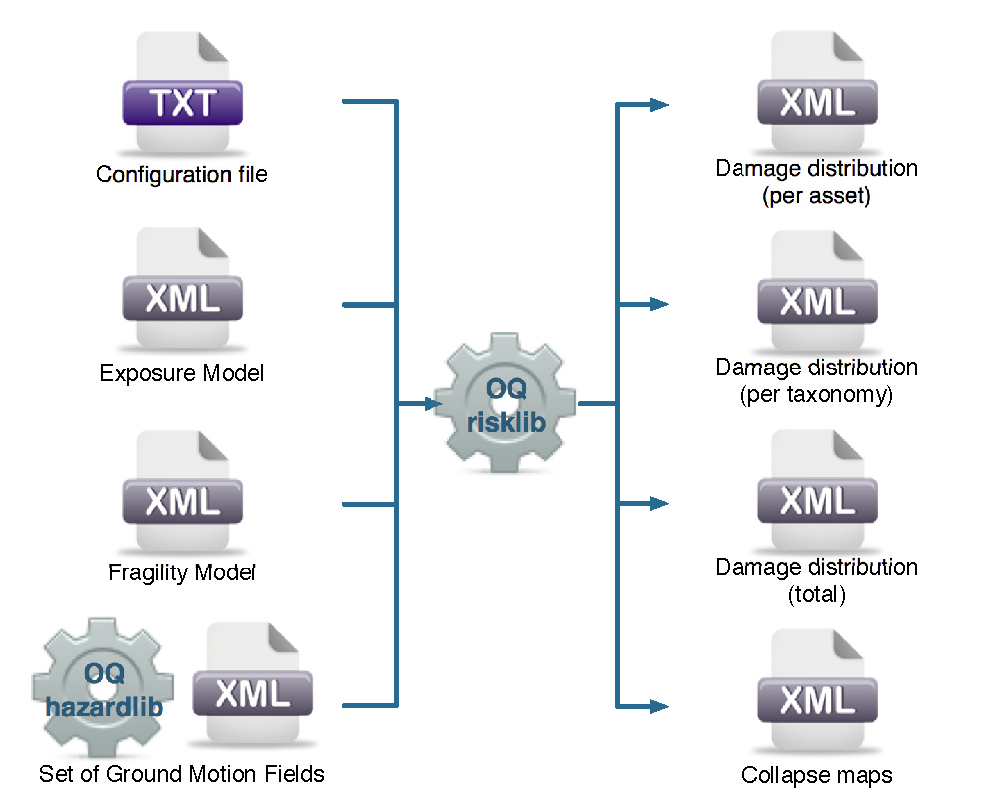
\includegraphics[width=9cm,height=7cm]{figures/risk/ScenarioDamage.pdf}
\caption{Scenario Damage Calculator input/output structure.}
\label{fig:ScnDamage}
\end{figure}

\subsection{Scenario Risk Assessment}
\index{OpenQuake-engine!Risk calculation workflows!Scenario Risk Assessment}
\label{subsec:workflow_scenario_risk}
This calculator computes loss maps and loss statistics due to a single seismic event, for a collection of assets. The hazard input can be a single ground motion field (e.g. the median distribution of ground motion in the region of interest) or a set of ground motion fields allowing the characterisation of the inter- and intra-event variability from the GMPE. It is noted that the hazard input can either be calculated using the hazard component of OpenQuake-engine (oq-hazardlib), or provided to the risk component iian external file following the respective Natural hazards' Risk Markup Language (NRML) schema (see \href{http://github.com/gem/oq-nrmllib}{oq-nrmllib}).
A vulnerability model is combined with the distribution of the ground motions at each asset location to calculate the loss distribution for each asset, as well as the statistics of the total loss throughout the region of interest. The required input files and resulting output files are depicted in Figure~\ref{fig:ScnRisk}.

\begin{figure}[ht]
\centering
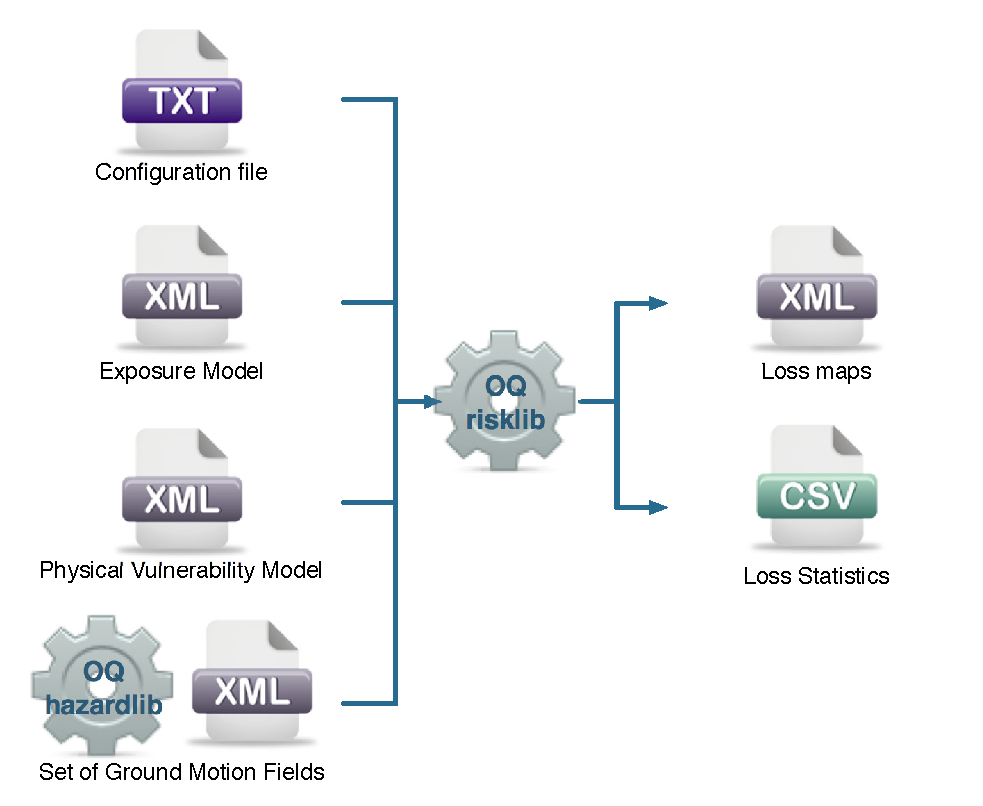
\includegraphics[width=9cm,height=7cm]{figures/risk/ScenarioRisk.pdf}
\caption{Scenario Risk Calculator input/output structure.}
\label{fig:ScnRisk}
\end{figure}

\subsection{Classical Probabilistic Seismic Damage Analysis}
\index{OpenQuake-engine!Risk calculation workflows!Classical Probabilistic Seismic Damage Analysis}
\label{subsec:workflow_classical_damage}
The classical PSHA-based damage calculator convolves through numerical integration, the damage state fragility functions for an asset with the seismic hazard curve at the location of the asset. The main results of this calculator are damage distribution statistics for each asset, which describe the expected fraction of buildings in each damage state. Furthermore, a probabilistic collapse map can be extracted giving the probability of collapse for each asset within the specified time period. Damage distribution aggregated by taxonomy or of the total portfolio (considering all assets in the exposure model) can not be extracted using this calculator, as the spatial correlation of the ground motion residuals is not taken into consideration. The input and output files involved in this calculator are presented in Figure~\ref{fig:ClassicalDamage}.

\begin{figure}[ht]
\centering
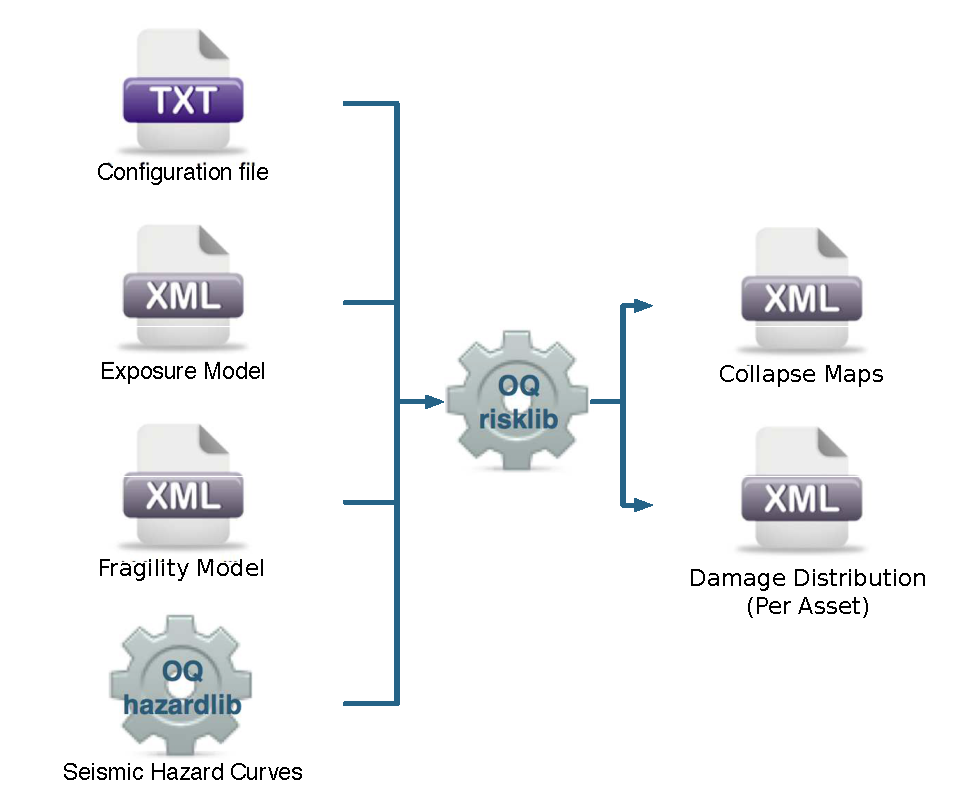
\includegraphics[width=9cm,height=7cm]{figures/risk/ClassicalDamage.pdf}
\caption{Classical PSHA-based Damage Calculator input/output structure.}
\label{fig:ClassicalDamage}
\end{figure}

\subsection{Classical Probabilistic Seismic Risk Analysis}
\index{OpenQuake-engine!Risk calculation workflows!Classical Probabilistic Seismic Risk Analysis}
\label{subsec:workflow_classical_risk}
The classical PSHA-based risk calculator convolves through numerical
integration, the probabilistic vulnerability functions for an asset with the
seismic hazard curve at the location of the asset, to give the loss
distribution for the asset within a specified time period. The calculator
requires the definition of an exposure model, a vulnerability model for each
loss type of interest with vulnerability functions for each taxonomy
represented in the exposure model, and hazard curves calculated in the region
of interest. Loss curves and loss maps can currently be calculated for five
different loss types using this calculator: structural losses, nonstructural
losses, contents losses, downtime losses, and occupant fatalities. The main
results of this calculator are loss exceedance curves for each asset, which
describe the probability of exceedance of different loss levels over the
specified time period, and loss maps for the region, which describe the loss
values that have a given probability of exceedance over the specified time

Unlike the probabilistic event-based risk calculator, an aggregate loss curve
(considering all assets in the exposure model) can not be extracted using this
calculator, as the correlation of the ground motion residuals and
vulnerability uncertainty is not taken into consideration in this calculator.

The hazard curves required for this calculator can be calculated by the
OpenQuake engine for all asset locations in the exposure model using the
classical PSHA approach \citep{cornell1968, mcguire1976}. The use of logic-
trees allows for the consideration of model uncertainty in the choice of a
ground motion prediction equation for the different tectonic region types in
the region. Unlike what was described in the previous calculator, a total loss
curve (considering all assets in the exposure model) can not be extracted
using this calculator, as the correlation of the ground motion residuals and
vulnerability uncertainty is not taken into consideration.

The required input files required for running a classical probabilistic risk
calculation and the resulting output files are depicted in Figure~\ref{fig:io-
structure-classical-risk}.

\begin{figure}[ht]
\centering
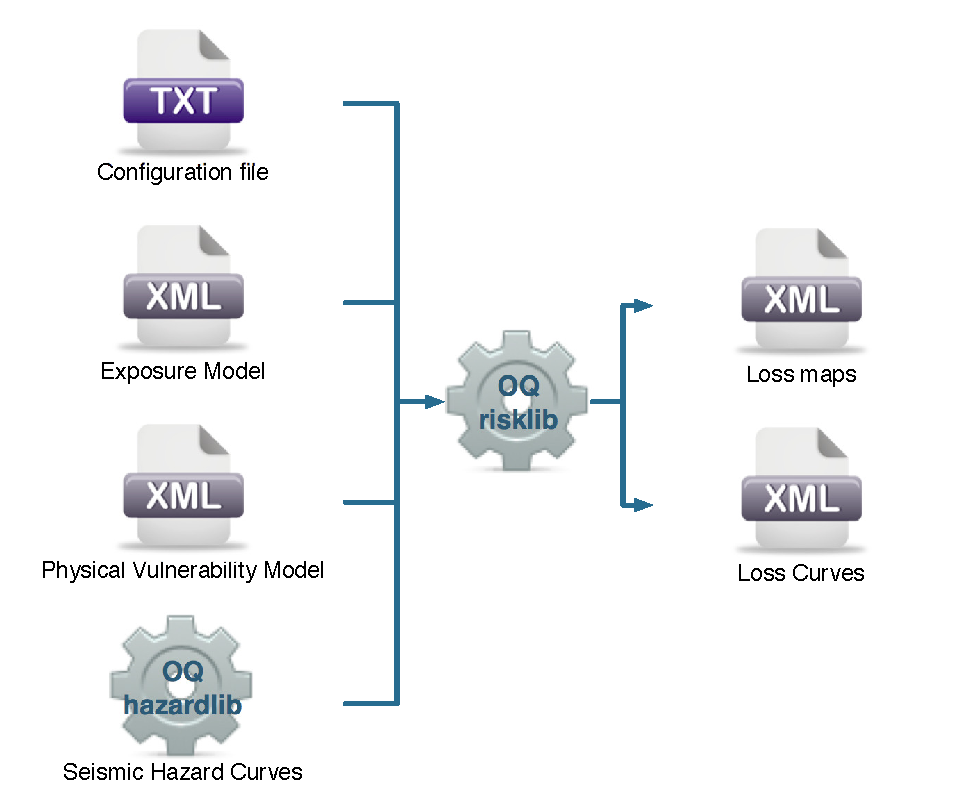
\includegraphics[width=9cm,height=7cm]{figures/risk/io-structure-classical-risk.pdf}
\caption{Classical PSHA-based Risk Calculator input/output structure.}
\label{fig:io-structure-classical-risk}
\end{figure}

\subsection{Event-Based Probabilistic Seismic Risk Analysis}
\index{OpenQuake-engine!Risk calculation workflows!Event-Based Probabilistic Seismic Risk Analysis}
\label{subsec:workflow_event_based_risk}
In this calculator, loss exceedance curves and loss maps for various return periods can be calculated, based on probabilistic seismic hazard, with an event-based approach. A large number of stochastic event sets are generated, and the associated ground motion fields for each event are used together with a vulnerability model to compute the individual (per asset) and total (sum of all the losses per event) losses. Then, this distribution of losses is employed to derive a loss exceedance curve per asset, as well as a total loss exceedance curve representative of the complete building portfolio. Furthermore, oq-risklib can also compute loss maps for various return periods by interpolating each individual loss curve with the respective probability of exceedance. In Figure~\ref{fig:ProbEvent}, the input/output scheme of this calculator is illustrated.

\begin{figure}[ht]
\centering
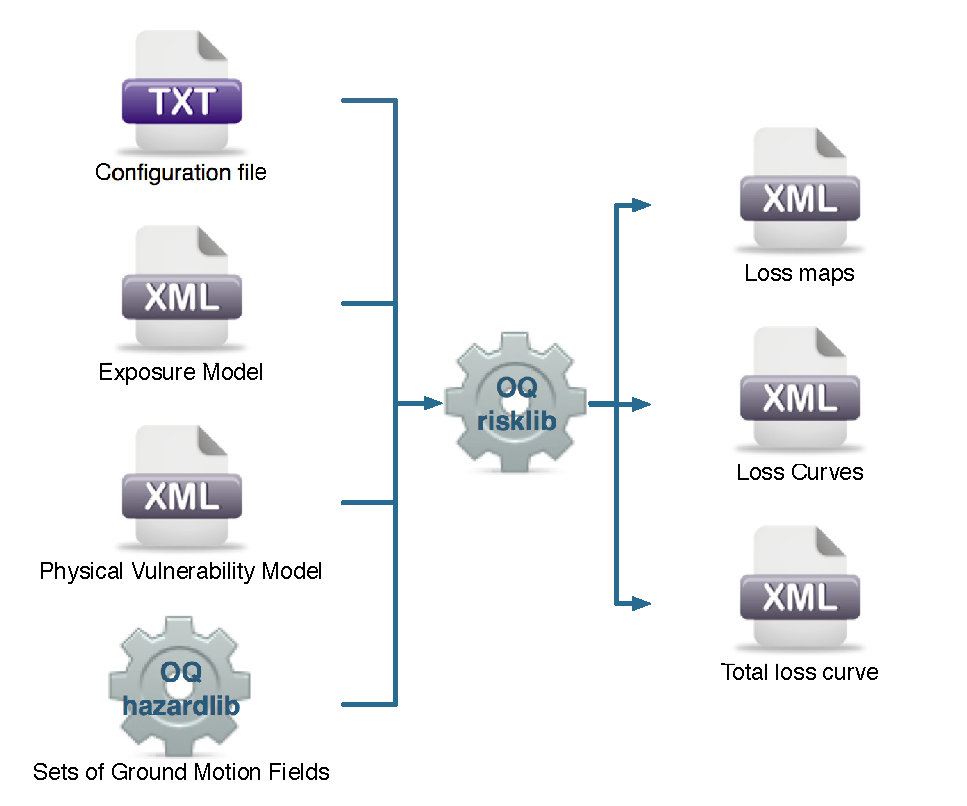
\includegraphics[width=9cm,height=7cm]{figures/risk/ProbEvent.pdf}
\caption{Probabilistic Event-based Risk Calculator input/output structure.}
\label{fig:ProbEvent}
\end{figure}

\subsection{Retrofit Benefit-Cost Ratio Analysis}
\index{OpenQuake-engine!Risk calculation workflows!Retrofit Benefit-Cost Ratio Analysis}
\label{subsec:workflow_benefit_cost}
This calculator represents a decision-support tool for deciding whether the
employment of retrofitting measures to a collection of existing buildings is
advantageous from an economical point of view. For this assessment, the
expected losses considering the original and retrofitted configuration of the
buildings are estimated, and the economic benefit due to the better seismic
design is divided by the retrofitting cost, leading to the benefit/cost ratio.
These loss curves are computed using the previously described  Classical PSHA-
based Risk calculator. The output of this calculator is a benefit/cost ratio
for each asset, in which a ratio above one indicates that employing  a
retrofitting intervention is economically viable.

In Figure~\ref{fig:io-structure-benefit-cost}, the input/output structure for
this calculator is depicted.

\begin{figure}[ht]
\centering
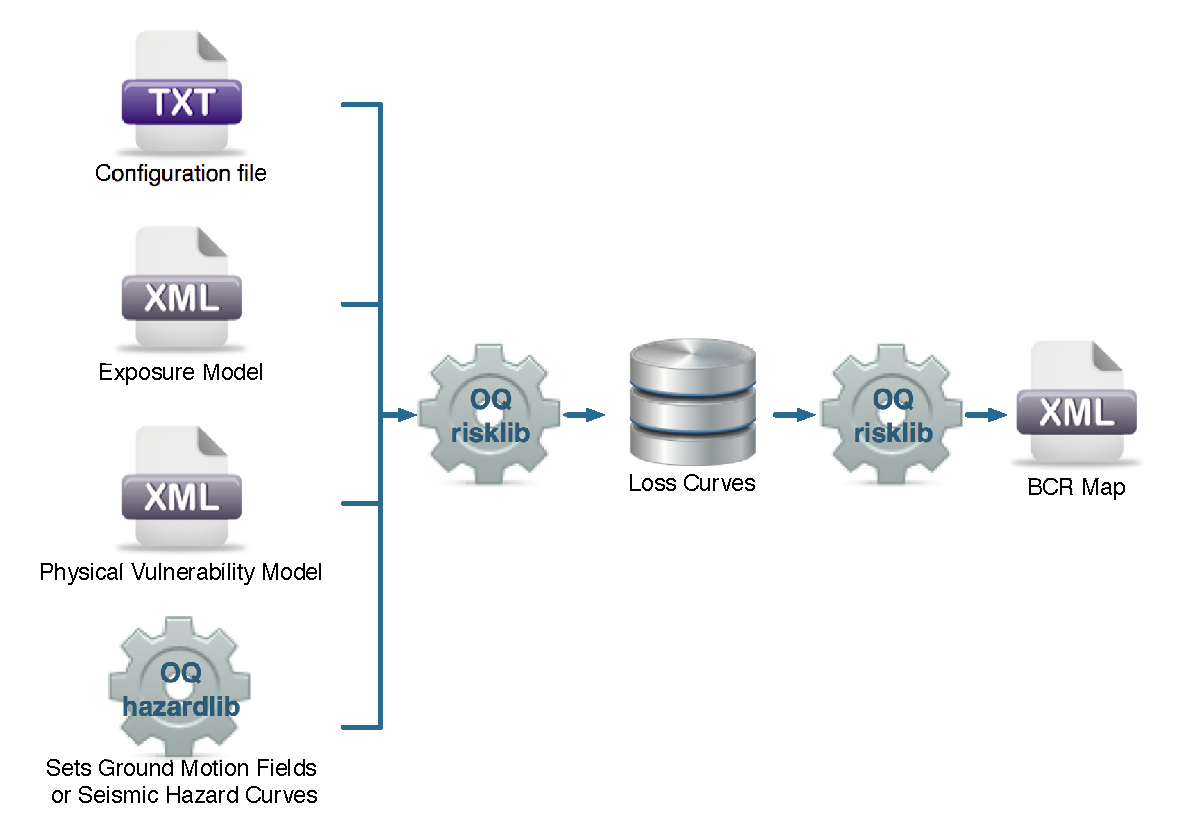
\includegraphics[width=10.5cm,height=7cm]{figures/risk/io-structure-benefit-cost.pdf}
\caption{Retrofitting Benefit/Cost Ratio Calculator input/output structure.}
\label{fig:io-structure-benefit-cost}
\end{figure}

\cleardoublepage